\documentclass[twoside]{book}

% Packages required by doxygen
\usepackage{fixltx2e}
\usepackage{calc}
\usepackage{doxygen}
\usepackage[export]{adjustbox} % also loads graphicx
\usepackage{graphicx}
\usepackage[utf8]{inputenc}
\usepackage{makeidx}
\usepackage{multicol}
\usepackage{multirow}
\PassOptionsToPackage{warn}{textcomp}
\usepackage{textcomp}
\usepackage[nointegrals]{wasysym}
\usepackage[table]{xcolor}

% Font selection
\usepackage[T1]{fontenc}
\usepackage[scaled=.90]{helvet}
\usepackage{courier}
\usepackage{amssymb}
\usepackage{sectsty}
\renewcommand{\familydefault}{\sfdefault}
\allsectionsfont{%
  \fontseries{bc}\selectfont%
  \color{darkgray}%
}
\renewcommand{\DoxyLabelFont}{%
  \fontseries{bc}\selectfont%
  \color{darkgray}%
}
\newcommand{\+}{\discretionary{\mbox{\scriptsize$\hookleftarrow$}}{}{}}

% Page & text layout
\usepackage{geometry}
\geometry{%
  a4paper,%
  top=2.5cm,%
  bottom=2.5cm,%
  left=2.5cm,%
  right=2.5cm%
}
\tolerance=750
\hfuzz=15pt
\hbadness=750
\setlength{\emergencystretch}{15pt}
\setlength{\parindent}{0cm}
\setlength{\parskip}{3ex plus 2ex minus 2ex}
\makeatletter
\renewcommand{\paragraph}{%
  \@startsection{paragraph}{4}{0ex}{-1.0ex}{1.0ex}{%
    \normalfont\normalsize\bfseries\SS@parafont%
  }%
}
\renewcommand{\subparagraph}{%
  \@startsection{subparagraph}{5}{0ex}{-1.0ex}{1.0ex}{%
    \normalfont\normalsize\bfseries\SS@subparafont%
  }%
}
\makeatother

% Headers & footers
\usepackage{fancyhdr}
\pagestyle{fancyplain}
\fancyhead[LE]{\fancyplain{}{\bfseries\thepage}}
\fancyhead[CE]{\fancyplain{}{}}
\fancyhead[RE]{\fancyplain{}{\bfseries\leftmark}}
\fancyhead[LO]{\fancyplain{}{\bfseries\rightmark}}
\fancyhead[CO]{\fancyplain{}{}}
\fancyhead[RO]{\fancyplain{}{\bfseries\thepage}}
\fancyfoot[LE]{\fancyplain{}{}}
\fancyfoot[CE]{\fancyplain{}{}}
\fancyfoot[RE]{\fancyplain{}{\bfseries\scriptsize Generated by Doxygen }}
\fancyfoot[LO]{\fancyplain{}{\bfseries\scriptsize Generated by Doxygen }}
\fancyfoot[CO]{\fancyplain{}{}}
\fancyfoot[RO]{\fancyplain{}{}}
\renewcommand{\footrulewidth}{0.4pt}
\renewcommand{\chaptermark}[1]{%
  \markboth{#1}{}%
}
\renewcommand{\sectionmark}[1]{%
  \markright{\thesection\ #1}%
}

% Indices & bibliography
\usepackage{natbib}
\usepackage[titles]{tocloft}
\setcounter{tocdepth}{3}
\setcounter{secnumdepth}{5}
\makeindex

% Hyperlinks (required, but should be loaded last)
\usepackage{ifpdf}
\ifpdf
  \usepackage[pdftex,pagebackref=true]{hyperref}
\else
  \usepackage[ps2pdf,pagebackref=true]{hyperref}
\fi
\hypersetup{%
  colorlinks=true,%
  linkcolor=blue,%
  citecolor=blue,%
  unicode%
}

% Custom commands
\newcommand{\clearemptydoublepage}{%
  \newpage{\pagestyle{empty}\cleardoublepage}%
}

\usepackage{caption}
\captionsetup{labelsep=space,justification=centering,font={bf},singlelinecheck=off,skip=4pt,position=top}

%===== C O N T E N T S =====

\begin{document}

% Titlepage & ToC
\hypersetup{pageanchor=false,
             bookmarksnumbered=true,
             pdfencoding=unicode
            }
\pagenumbering{roman}
\begin{titlepage}
\vspace*{7cm}
\begin{center}%
{\Large S\+O\+Lar-\/\+Fighter }\\
\vspace*{1cm}
{\large Generated by Doxygen 1.8.11}\\
\end{center}
\end{titlepage}
\clearemptydoublepage
\tableofcontents
\clearemptydoublepage
\pagenumbering{arabic}
\hypersetup{pageanchor=true}

%--- Begin generated contents ---
\chapter{Main Page}
\label{index}\hypertarget{index}{}Projekt zaliczeniowy z S\+Z\+P\+C++ a zarazem odrobina dobrej zabawy -\/ symulator lotu myśliwcem kosmicznym w 3D (na bazie allegro4 i alleggl). \begin{DoxyAuthor}{Autor}
Aleksander Szpakiewicz-\/\+Szatan 
\end{DoxyAuthor}
\begin{DoxyDate}{Data}
2016.\+12.\+29 
\end{DoxyDate}
\begin{DoxyVersion}{Wersja}
alfa 1.\+0.\+3 
\end{DoxyVersion}

\chapter{Hierarchical Index}
\section{Hierarchia klas}
Ta lista dziedziczenia posortowana jest z grubsza, choć nie całkowicie, alfabetycznie\+:\begin{DoxyCompactList}
\item \contentsline{section}{Renderable}{\pageref{class_renderable}}{}
\begin{DoxyCompactList}
\item \contentsline{section}{Orb}{\pageref{class_orb}}{}
\item \contentsline{section}{Simple\+Object}{\pageref{class_simple_object}}{}
\begin{DoxyCompactList}
\item \contentsline{section}{Camera}{\pageref{class_camera}}{}
\item \contentsline{section}{Object}{\pageref{class_object}}{}
\begin{DoxyCompactList}
\item \contentsline{section}{Mobile\+Object}{\pageref{class_mobile_object}}{}
\end{DoxyCompactList}
\end{DoxyCompactList}
\item \contentsline{section}{Star}{\pageref{class_star}}{}
\end{DoxyCompactList}
\item \contentsline{section}{Simulator}{\pageref{class_simulator}}{}
\end{DoxyCompactList}

\chapter{Class Index}
\section{Struktury danych}
Tutaj znajdują się struktury danych wraz z ich krótkimi opisami\+:\begin{DoxyCompactList}
\item\contentsline{section}{\hyperlink{class_camera}{Camera} }{\pageref{class_camera}}{}
\item\contentsline{section}{\hyperlink{class_mobile_object}{Mobile\+Object} }{\pageref{class_mobile_object}}{}
\item\contentsline{section}{\hyperlink{class_object}{Object} }{\pageref{class_object}}{}
\item\contentsline{section}{\hyperlink{class_orb}{Orb} }{\pageref{class_orb}}{}
\item\contentsline{section}{\hyperlink{class_renderable}{Renderable} }{\pageref{class_renderable}}{}
\item\contentsline{section}{\hyperlink{class_simple_object}{Simple\+Object} }{\pageref{class_simple_object}}{}
\item\contentsline{section}{\hyperlink{class_simulator}{Simulator} }{\pageref{class_simulator}}{}
\item\contentsline{section}{\hyperlink{class_star}{Star} }{\pageref{class_star}}{}
\end{DoxyCompactList}

\chapter{Class Documentation}
\hypertarget{class_camera}{}\section{Dokumentacja klasy Camera}
\label{class_camera}\index{Camera@{Camera}}


{\ttfamily \#include $<$camera.\+hpp$>$}



Diagram dziedziczenia dla Camera
\nopagebreak
\begin{figure}[H]
\begin{center}
\leavevmode
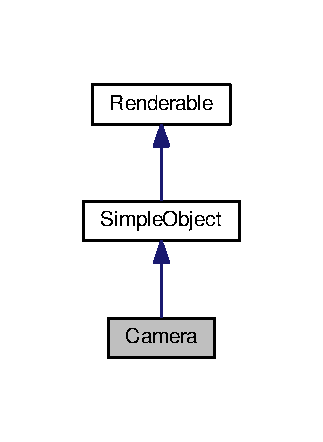
\includegraphics[width=155pt]{class_camera__inherit__graph}
\end{center}
\end{figure}


Diagram współpracy dla Camera\+:
\nopagebreak
\begin{figure}[H]
\begin{center}
\leavevmode
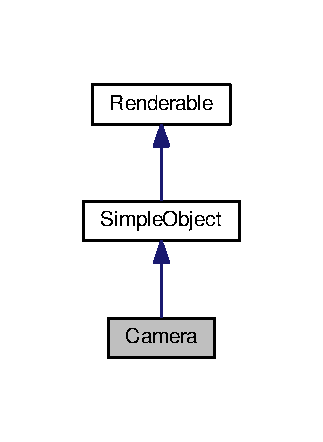
\includegraphics[width=155pt]{class_camera__coll__graph}
\end{center}
\end{figure}
\subsection*{Metody publiczne}
\begin{DoxyCompactItemize}
\item 
\hyperlink{class_camera_aa4fab6c2c09702f8e70d0688ea90c0ae}{Camera} (double x, double y, double z, double yaw, double pitch, double roll, double fov\+\_\+x, double fov\+\_\+y, double render\+\_\+dist, B\+I\+T\+M\+AP $\ast$scr, double res\+\_\+x, double res\+\_\+y)
\item 
double \hyperlink{class_camera_ad85cea48af89cad24edc3eb2bdcdf7ee}{get\+\_\+x\+\_\+sin\+\_\+fov\+\_\+const} () const 
\item 
double \hyperlink{class_camera_a87266e92e70522c3d0e1c397b4ada1af}{get\+\_\+y\+\_\+sin\+\_\+fov\+\_\+const} () const 
\item 
double \hyperlink{class_camera_a1bda457bae36f6a8d0ecf29bd0ec19a9}{get\+\_\+render\+\_\+dist} () const 
\item 
unsigned \hyperlink{class_camera_a744c0732cff592644a4f0e62654d1d10}{get\+\_\+res\+\_\+x} () const 
\item 
unsigned \hyperlink{class_camera_a7d62c7d80c97dc2e703544e7280a5208}{get\+\_\+res\+\_\+y} () const 
\item 
unsigned \hyperlink{class_camera_aa106361d6bab194723cb746c22df8cbe}{get\+\_\+res\+\_\+x2} () const 
\item 
unsigned \hyperlink{class_camera_af0d5d16f478c68fdc8f3bfda7db0ad72}{get\+\_\+res\+\_\+y2} () const 
\item 
double \hyperlink{class_camera_a3537564f96a44b3480d5581c7fec5576}{get\+\_\+fov\+\_\+x2} () const 
\item 
double \hyperlink{class_camera_a160845f2c2da8ef18459b4fc1d5c3929}{get\+\_\+fov\+\_\+y2} () const 
\item 
void \hyperlink{class_camera_a02a92079d7a27b0801611c280b17002b}{putpixel} (int xx, int yy, int col) const 
\item 
void \hyperlink{class_camera_adfd2ffd6a173e3125a220164687d88b1}{ellipsefill} (int xx, int yy, int rad\+\_\+x, int rad\+\_\+y, int col) const 
\item 
virtual void \hyperlink{class_camera_ab521598bed84988be95a89dfcdd9f1aa}{update} (double dt)
\item 
void {\bfseries accel\+\_\+line} (double a)\hypertarget{class_camera_aa8322375b803f39cb2071be302de4d6e}{}\label{class_camera_aa8322375b803f39cb2071be302de4d6e}

\item 
void {\bfseries accel\+\_\+deg} (double ayaw, double apitch)\hypertarget{class_camera_a301f57ac80bd72485ba854cc08133a82}{}\label{class_camera_a301f57ac80bd72485ba854cc08133a82}

\item 
void {\bfseries accel\+\_\+roll} (double aroll)\hypertarget{class_camera_a7cdb0dd64bb945b4505bc9e8f3ceb980}{}\label{class_camera_a7cdb0dd64bb945b4505bc9e8f3ceb980}

\end{DoxyCompactItemize}
\subsection*{Atrybuty chronione}
\begin{DoxyCompactItemize}
\item 
double {\bfseries fov\+\_\+x2\+\_\+}\hypertarget{class_camera_ad6f9e802013ee6a2b213b9d10c98486d}{}\label{class_camera_ad6f9e802013ee6a2b213b9d10c98486d}

\item 
double {\bfseries fov\+\_\+y2\+\_\+}\hypertarget{class_camera_ad7cca2cccd8e80f609b4286b80790a32}{}\label{class_camera_ad7cca2cccd8e80f609b4286b80790a32}

\item 
double {\bfseries render\+\_\+dist\+\_\+}\hypertarget{class_camera_afa21bbf24f05d8de6f627c69c9483f51}{}\label{class_camera_afa21bbf24f05d8de6f627c69c9483f51}

\item 
B\+I\+T\+M\+AP $\ast$ {\bfseries scr\+\_\+}\hypertarget{class_camera_a894521c08c09d8aceafadb9e936f6078}{}\label{class_camera_a894521c08c09d8aceafadb9e936f6078}

\item 
unsigned {\bfseries res\+\_\+x\+\_\+}\hypertarget{class_camera_a2802feb57ae1946b07bbdba556fcbeb7}{}\label{class_camera_a2802feb57ae1946b07bbdba556fcbeb7}

\item 
unsigned {\bfseries res\+\_\+y\+\_\+}\hypertarget{class_camera_a03472c7407e3cc29e7c4b5917bfcd6ee}{}\label{class_camera_a03472c7407e3cc29e7c4b5917bfcd6ee}

\item 
unsigned {\bfseries res\+\_\+x2\+\_\+}\hypertarget{class_camera_a42e9c3892b3afc9a24001a3c537da592}{}\label{class_camera_a42e9c3892b3afc9a24001a3c537da592}

\item 
unsigned {\bfseries res\+\_\+y2\+\_\+}\hypertarget{class_camera_a0a7acab770bd82600f504cd0325b3b00}{}\label{class_camera_a0a7acab770bd82600f504cd0325b3b00}

\item 
double {\bfseries x\+\_\+sin\+\_\+fov\+\_\+const\+\_\+}\hypertarget{class_camera_a7ffda0b88dafdbd3156d59bbec896bd0}{}\label{class_camera_a7ffda0b88dafdbd3156d59bbec896bd0}

\item 
double {\bfseries y\+\_\+sin\+\_\+fov\+\_\+const\+\_\+}\hypertarget{class_camera_a6489f19c9ae8cb252513bee7c76ea922}{}\label{class_camera_a6489f19c9ae8cb252513bee7c76ea922}

\item 
double {\bfseries vx\+\_\+}\hypertarget{class_camera_a7383b28a310ea2664874fbabe5e66e38}{}\label{class_camera_a7383b28a310ea2664874fbabe5e66e38}

\item 
double {\bfseries vy\+\_\+}\hypertarget{class_camera_aba5e551b383324cf19e4dfdff103229a}{}\label{class_camera_aba5e551b383324cf19e4dfdff103229a}

\item 
double {\bfseries vz\+\_\+}\hypertarget{class_camera_ae5770bf3fd53854d5dd9cdcbc18fdab3}{}\label{class_camera_ae5770bf3fd53854d5dd9cdcbc18fdab3}

\item 
double {\bfseries vyaw\+\_\+}\hypertarget{class_camera_af5a43904926f58b8fe1b3da391cdc9ea}{}\label{class_camera_af5a43904926f58b8fe1b3da391cdc9ea}

\item 
double {\bfseries vpitch\+\_\+}\hypertarget{class_camera_a0edd07cc2b7b294fddaf29dec22fc63a}{}\label{class_camera_a0edd07cc2b7b294fddaf29dec22fc63a}

\item 
double {\bfseries vroll\+\_\+}\hypertarget{class_camera_ad356a82282afe866ebf827eef7b9e1b3}{}\label{class_camera_ad356a82282afe866ebf827eef7b9e1b3}

\end{DoxyCompactItemize}


\subsection{Opis szczegółowy}
Klasa kamery -\/ punktu widzenia gracza 

\subsection{Dokumentacja konstruktora i destruktora}
\index{Camera@{Camera}!Camera@{Camera}}
\index{Camera@{Camera}!Camera@{Camera}}
\subsubsection[{\texorpdfstring{Camera(double x, double y, double z, double yaw, double pitch, double roll, double fov\+\_\+x, double fov\+\_\+y, double render\+\_\+dist, B\+I\+T\+M\+A\+P $\ast$scr, double res\+\_\+x, double res\+\_\+y)}{Camera(double x, double y, double z, double yaw, double pitch, double roll, double fov_x, double fov_y, double render_dist, BITMAP *scr, double res_x, double res_y)}}]{\setlength{\rightskip}{0pt plus 5cm}Camera\+::\+Camera (
\begin{DoxyParamCaption}
\item[{double}]{x, }
\item[{double}]{y, }
\item[{double}]{z, }
\item[{double}]{yaw, }
\item[{double}]{pitch, }
\item[{double}]{roll, }
\item[{double}]{fov\+\_\+x, }
\item[{double}]{fov\+\_\+y, }
\item[{double}]{render\+\_\+dist, }
\item[{B\+I\+T\+M\+AP $\ast$}]{scr, }
\item[{double}]{res\+\_\+x, }
\item[{double}]{res\+\_\+y}
\end{DoxyParamCaption}
)}\hypertarget{class_camera_aa4fab6c2c09702f8e70d0688ea90c0ae}{}\label{class_camera_aa4fab6c2c09702f8e70d0688ea90c0ae}
Konstruktor klasy \hyperlink{class_camera}{Camera} 
\begin{DoxyParams}{Parametry}
{\em x} & -\/ położenie w osi x \\
\hline
{\em y} & -\/ położenie w osi y \\
\hline
{\em z} & -\/ położenie w osi z \\
\hline
{\em yaw} & -\/ obrót w osi z \\
\hline
{\em pitch} & -\/ obrót w osi xy \\
\hline
{\em roll} & -\/ obrót wokół własnej osi \\
\hline
{\em fov\+\_\+x} & -\/ szerokość kątowa pola widzenia w poziomie \\
\hline
{\em fov\+\_\+y} & -\/ szerokość kątowa pola widzenia w pionie \\
\hline
{\em render\+\_\+dist} & -\/ zasięg rysowania \\
\hline
{\em scr} & -\/ bitmapa do której rysuje kamera (z założenia ekran) \\
\hline
{\em res\+\_\+x} & -\/ rozdzielczość pozioma bitmapy \\
\hline
{\em res\+\_\+y} & -\/ rozdzielczość pionowa bitmapy \\
\hline
\end{DoxyParams}
\begin{DoxyReturn}{Zwraca}
obiekt typu \hyperlink{class_camera}{Camera} 
\end{DoxyReturn}


\subsection{Dokumentacja funkcji składowych}
\index{Camera@{Camera}!ellipsefill@{ellipsefill}}
\index{ellipsefill@{ellipsefill}!Camera@{Camera}}
\subsubsection[{\texorpdfstring{ellipsefill(int xx, int yy, int rad\+\_\+x, int rad\+\_\+y, int col) const }{ellipsefill(int xx, int yy, int rad_x, int rad_y, int col) const }}]{\setlength{\rightskip}{0pt plus 5cm}void Camera\+::ellipsefill (
\begin{DoxyParamCaption}
\item[{int}]{xx, }
\item[{int}]{yy, }
\item[{int}]{rad\+\_\+x, }
\item[{int}]{rad\+\_\+y, }
\item[{int}]{col}
\end{DoxyParamCaption}
) const\hspace{0.3cm}{\ttfamily [inline]}}\hypertarget{class_camera_adfd2ffd6a173e3125a220164687d88b1}{}\label{class_camera_adfd2ffd6a173e3125a220164687d88b1}
\begin{DoxyReturn}{Zwraca}
rysuje wypełnioną elipsę na ekranie bez bezpośredniego dostępu do prywatnej bitmapy 
\end{DoxyReturn}
\index{Camera@{Camera}!get\+\_\+fov\+\_\+x2@{get\+\_\+fov\+\_\+x2}}
\index{get\+\_\+fov\+\_\+x2@{get\+\_\+fov\+\_\+x2}!Camera@{Camera}}
\subsubsection[{\texorpdfstring{get\+\_\+fov\+\_\+x2() const }{get_fov_x2() const }}]{\setlength{\rightskip}{0pt plus 5cm}double Camera\+::get\+\_\+fov\+\_\+x2 (
\begin{DoxyParamCaption}
{}
\end{DoxyParamCaption}
) const\hspace{0.3cm}{\ttfamily [inline]}}\hypertarget{class_camera_a3537564f96a44b3480d5581c7fec5576}{}\label{class_camera_a3537564f96a44b3480d5581c7fec5576}
\begin{DoxyReturn}{Zwraca}
szerokość kątowa pola widzenia w poziomie 
\end{DoxyReturn}
\index{Camera@{Camera}!get\+\_\+fov\+\_\+y2@{get\+\_\+fov\+\_\+y2}}
\index{get\+\_\+fov\+\_\+y2@{get\+\_\+fov\+\_\+y2}!Camera@{Camera}}
\subsubsection[{\texorpdfstring{get\+\_\+fov\+\_\+y2() const }{get_fov_y2() const }}]{\setlength{\rightskip}{0pt plus 5cm}double Camera\+::get\+\_\+fov\+\_\+y2 (
\begin{DoxyParamCaption}
{}
\end{DoxyParamCaption}
) const\hspace{0.3cm}{\ttfamily [inline]}}\hypertarget{class_camera_a160845f2c2da8ef18459b4fc1d5c3929}{}\label{class_camera_a160845f2c2da8ef18459b4fc1d5c3929}
\begin{DoxyReturn}{Zwraca}
szerokość kątowa pola widzenia w pionie 
\end{DoxyReturn}
\index{Camera@{Camera}!get\+\_\+render\+\_\+dist@{get\+\_\+render\+\_\+dist}}
\index{get\+\_\+render\+\_\+dist@{get\+\_\+render\+\_\+dist}!Camera@{Camera}}
\subsubsection[{\texorpdfstring{get\+\_\+render\+\_\+dist() const }{get_render_dist() const }}]{\setlength{\rightskip}{0pt plus 5cm}double Camera\+::get\+\_\+render\+\_\+dist (
\begin{DoxyParamCaption}
{}
\end{DoxyParamCaption}
) const\hspace{0.3cm}{\ttfamily [inline]}}\hypertarget{class_camera_a1bda457bae36f6a8d0ecf29bd0ec19a9}{}\label{class_camera_a1bda457bae36f6a8d0ecf29bd0ec19a9}
\begin{DoxyReturn}{Zwraca}
zasięg renderowania 
\end{DoxyReturn}
\index{Camera@{Camera}!get\+\_\+res\+\_\+x@{get\+\_\+res\+\_\+x}}
\index{get\+\_\+res\+\_\+x@{get\+\_\+res\+\_\+x}!Camera@{Camera}}
\subsubsection[{\texorpdfstring{get\+\_\+res\+\_\+x() const }{get_res_x() const }}]{\setlength{\rightskip}{0pt plus 5cm}unsigned Camera\+::get\+\_\+res\+\_\+x (
\begin{DoxyParamCaption}
{}
\end{DoxyParamCaption}
) const\hspace{0.3cm}{\ttfamily [inline]}}\hypertarget{class_camera_a744c0732cff592644a4f0e62654d1d10}{}\label{class_camera_a744c0732cff592644a4f0e62654d1d10}
\begin{DoxyReturn}{Zwraca}
rozdzielczość pozioma ekranu 
\end{DoxyReturn}
\index{Camera@{Camera}!get\+\_\+res\+\_\+x2@{get\+\_\+res\+\_\+x2}}
\index{get\+\_\+res\+\_\+x2@{get\+\_\+res\+\_\+x2}!Camera@{Camera}}
\subsubsection[{\texorpdfstring{get\+\_\+res\+\_\+x2() const }{get_res_x2() const }}]{\setlength{\rightskip}{0pt plus 5cm}unsigned Camera\+::get\+\_\+res\+\_\+x2 (
\begin{DoxyParamCaption}
{}
\end{DoxyParamCaption}
) const\hspace{0.3cm}{\ttfamily [inline]}}\hypertarget{class_camera_aa106361d6bab194723cb746c22df8cbe}{}\label{class_camera_aa106361d6bab194723cb746c22df8cbe}
\begin{DoxyReturn}{Zwraca}
rozdzielczość pozioma połówki ekranu 
\end{DoxyReturn}
\index{Camera@{Camera}!get\+\_\+res\+\_\+y@{get\+\_\+res\+\_\+y}}
\index{get\+\_\+res\+\_\+y@{get\+\_\+res\+\_\+y}!Camera@{Camera}}
\subsubsection[{\texorpdfstring{get\+\_\+res\+\_\+y() const }{get_res_y() const }}]{\setlength{\rightskip}{0pt plus 5cm}unsigned Camera\+::get\+\_\+res\+\_\+y (
\begin{DoxyParamCaption}
{}
\end{DoxyParamCaption}
) const\hspace{0.3cm}{\ttfamily [inline]}}\hypertarget{class_camera_a7d62c7d80c97dc2e703544e7280a5208}{}\label{class_camera_a7d62c7d80c97dc2e703544e7280a5208}
\begin{DoxyReturn}{Zwraca}
rozdzielczość pionowa ekranu 
\end{DoxyReturn}
\index{Camera@{Camera}!get\+\_\+res\+\_\+y2@{get\+\_\+res\+\_\+y2}}
\index{get\+\_\+res\+\_\+y2@{get\+\_\+res\+\_\+y2}!Camera@{Camera}}
\subsubsection[{\texorpdfstring{get\+\_\+res\+\_\+y2() const }{get_res_y2() const }}]{\setlength{\rightskip}{0pt plus 5cm}unsigned Camera\+::get\+\_\+res\+\_\+y2 (
\begin{DoxyParamCaption}
{}
\end{DoxyParamCaption}
) const\hspace{0.3cm}{\ttfamily [inline]}}\hypertarget{class_camera_af0d5d16f478c68fdc8f3bfda7db0ad72}{}\label{class_camera_af0d5d16f478c68fdc8f3bfda7db0ad72}
\begin{DoxyReturn}{Zwraca}
rozdzielczość pionowa połówki ekranu 
\end{DoxyReturn}
\index{Camera@{Camera}!get\+\_\+x\+\_\+sin\+\_\+fov\+\_\+const@{get\+\_\+x\+\_\+sin\+\_\+fov\+\_\+const}}
\index{get\+\_\+x\+\_\+sin\+\_\+fov\+\_\+const@{get\+\_\+x\+\_\+sin\+\_\+fov\+\_\+const}!Camera@{Camera}}
\subsubsection[{\texorpdfstring{get\+\_\+x\+\_\+sin\+\_\+fov\+\_\+const() const }{get_x_sin_fov_const() const }}]{\setlength{\rightskip}{0pt plus 5cm}double Camera\+::get\+\_\+x\+\_\+sin\+\_\+fov\+\_\+const (
\begin{DoxyParamCaption}
{}
\end{DoxyParamCaption}
) const\hspace{0.3cm}{\ttfamily [inline]}}\hypertarget{class_camera_ad85cea48af89cad24edc3eb2bdcdf7ee}{}\label{class_camera_ad85cea48af89cad24edc3eb2bdcdf7ee}
\begin{DoxyReturn}{Zwraca}
stała niezbędna do wyznaczania położeń gwiazd w osi poziomej ekranu 
\end{DoxyReturn}
\index{Camera@{Camera}!get\+\_\+y\+\_\+sin\+\_\+fov\+\_\+const@{get\+\_\+y\+\_\+sin\+\_\+fov\+\_\+const}}
\index{get\+\_\+y\+\_\+sin\+\_\+fov\+\_\+const@{get\+\_\+y\+\_\+sin\+\_\+fov\+\_\+const}!Camera@{Camera}}
\subsubsection[{\texorpdfstring{get\+\_\+y\+\_\+sin\+\_\+fov\+\_\+const() const }{get_y_sin_fov_const() const }}]{\setlength{\rightskip}{0pt plus 5cm}double Camera\+::get\+\_\+y\+\_\+sin\+\_\+fov\+\_\+const (
\begin{DoxyParamCaption}
{}
\end{DoxyParamCaption}
) const\hspace{0.3cm}{\ttfamily [inline]}}\hypertarget{class_camera_a87266e92e70522c3d0e1c397b4ada1af}{}\label{class_camera_a87266e92e70522c3d0e1c397b4ada1af}
\begin{DoxyReturn}{Zwraca}
stała niezbędna do wyznaczania położeń gwiazd w osi pionowej ekranu 
\end{DoxyReturn}
\index{Camera@{Camera}!putpixel@{putpixel}}
\index{putpixel@{putpixel}!Camera@{Camera}}
\subsubsection[{\texorpdfstring{putpixel(int xx, int yy, int col) const }{putpixel(int xx, int yy, int col) const }}]{\setlength{\rightskip}{0pt plus 5cm}void Camera\+::putpixel (
\begin{DoxyParamCaption}
\item[{int}]{xx, }
\item[{int}]{yy, }
\item[{int}]{col}
\end{DoxyParamCaption}
) const\hspace{0.3cm}{\ttfamily [inline]}}\hypertarget{class_camera_a02a92079d7a27b0801611c280b17002b}{}\label{class_camera_a02a92079d7a27b0801611c280b17002b}
\begin{DoxyReturn}{Zwraca}
umieszcza piksel na ekranie bez bezpośredniego dostępu do prywatnej bitmapy 
\end{DoxyReturn}
\index{Camera@{Camera}!update@{update}}
\index{update@{update}!Camera@{Camera}}
\subsubsection[{\texorpdfstring{update(double dt)}{update(double dt)}}]{\setlength{\rightskip}{0pt plus 5cm}void Camera\+::update (
\begin{DoxyParamCaption}
\item[{double}]{dt}
\end{DoxyParamCaption}
)\hspace{0.3cm}{\ttfamily [virtual]}}\hypertarget{class_camera_ab521598bed84988be95a89dfcdd9f1aa}{}\label{class_camera_ab521598bed84988be95a89dfcdd9f1aa}
Aktualizuje położenie zmienne w czasie 
\begin{DoxyParams}{Parametry}
{\em dt} & -\/ krok czasowy \\
\hline
\end{DoxyParams}


Implementuje \hyperlink{class_simple_object}{Simple\+Object}.



Dokumentacja dla tej klasy została wygenerowana z plików\+:\begin{DoxyCompactItemize}
\item 
src/camera.\+hpp\item 
src/camera.\+cpp\end{DoxyCompactItemize}

\hypertarget{class_mobile_object}{}\section{Mobile\+Object Class Reference}
\label{class_mobile_object}\index{Mobile\+Object@{Mobile\+Object}}


Inheritance diagram for Mobile\+Object\+:\nopagebreak
\begin{figure}[H]
\begin{center}
\leavevmode
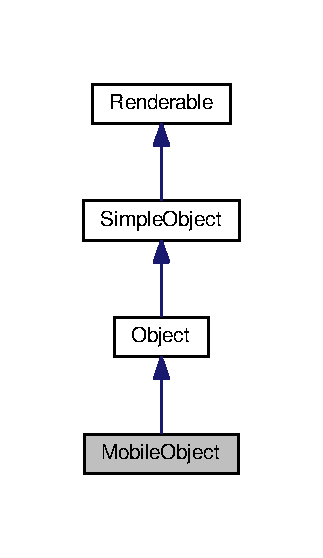
\includegraphics[width=155pt]{class_mobile_object__inherit__graph}
\end{center}
\end{figure}


Collaboration diagram for Mobile\+Object\+:\nopagebreak
\begin{figure}[H]
\begin{center}
\leavevmode
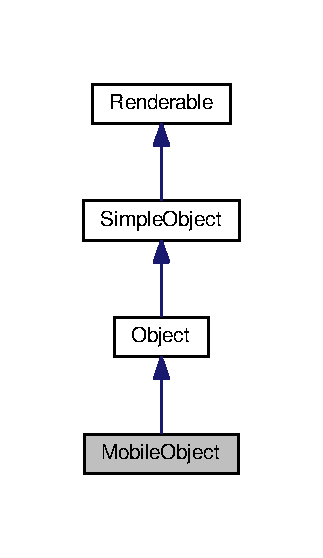
\includegraphics[width=155pt]{class_mobile_object__coll__graph}
\end{center}
\end{figure}
\subsection*{Additional Inherited Members}


The documentation for this class was generated from the following file\+:\begin{DoxyCompactItemize}
\item 
src/mobile\+\_\+object.\+hpp\end{DoxyCompactItemize}

\hypertarget{class_object}{}\section{Object Class Reference}
\label{class_object}\index{Object@{Object}}


Inheritance diagram for Object\+:\nopagebreak
\begin{figure}[H]
\begin{center}
\leavevmode
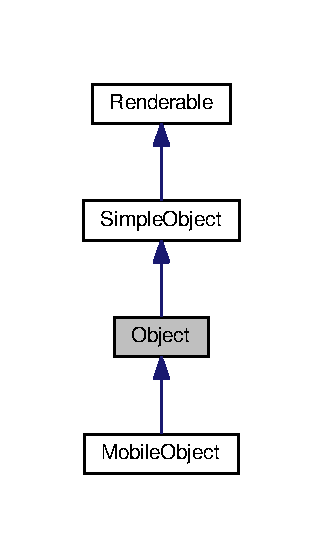
\includegraphics[width=155pt]{class_object__inherit__graph}
\end{center}
\end{figure}


Collaboration diagram for Object\+:\nopagebreak
\begin{figure}[H]
\begin{center}
\leavevmode
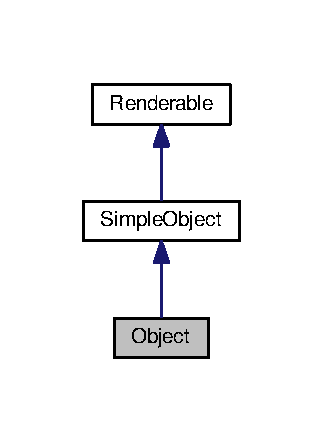
\includegraphics[width=155pt]{class_object__coll__graph}
\end{center}
\end{figure}
\subsection*{Public Member Functions}
\begin{DoxyCompactItemize}
\item 
{\bfseries Object} (double x, double y, double z, double yaw, double pitch, double roll, double size\+\_\+x, double size\+\_\+y, double size\+\_\+z)\hypertarget{class_object_a7183ffb5489cedf54629055db8d57ff5}{}\label{class_object_a7183ffb5489cedf54629055db8d57ff5}

\item 
virtual bool {\bfseries is\+\_\+visible} (const \hyperlink{class_camera}{Camera} $\ast$camera)\hypertarget{class_object_ab4c6e9456feda15cf49b85ce196666e6}{}\label{class_object_ab4c6e9456feda15cf49b85ce196666e6}

\item 
virtual void {\bfseries render} (const \hyperlink{class_camera}{Camera} $\ast$camera)\hypertarget{class_object_a7b6ef90438e4b82e479197bc6261c25a}{}\label{class_object_a7b6ef90438e4b82e479197bc6261c25a}

\end{DoxyCompactItemize}
\subsection*{Additional Inherited Members}


The documentation for this class was generated from the following files\+:\begin{DoxyCompactItemize}
\item 
src/object.\+hpp\item 
src/object.\+cpp\end{DoxyCompactItemize}

\hypertarget{class_orb}{}\section{Orb Class Reference}
\label{class_orb}\index{Orb@{Orb}}


{\ttfamily \#include $<$orb.\+hpp$>$}



Inheritance diagram for Orb\+:\nopagebreak
\begin{figure}[H]
\begin{center}
\leavevmode
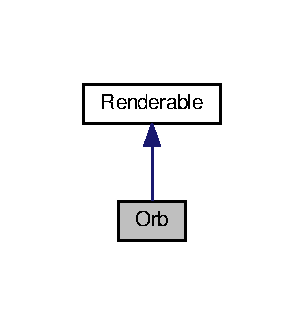
\includegraphics[width=146pt]{class_orb__inherit__graph}
\end{center}
\end{figure}


Collaboration diagram for Orb\+:\nopagebreak
\begin{figure}[H]
\begin{center}
\leavevmode
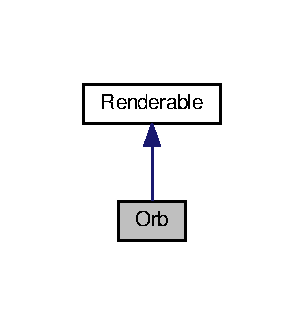
\includegraphics[width=146pt]{class_orb__coll__graph}
\end{center}
\end{figure}
\subsection*{Public Member Functions}
\begin{DoxyCompactItemize}
\item 
\hyperlink{class_orb_a3407825c339b82eaff3b59738670350a}{Orb} (double m, double radius, int color, double r=0, double alfa=0, double z=0, double yaw=0, double pitch=0, double roll=0, double vr=0, double valfa=0, double vz=0, double vyaw=0, double vpitch=0, double vroll=0)
\item 
\hyperlink{class_orb_adeeb210501049c0d1a2e1a5c4761c8c8}{Orb} (const \hyperlink{class_orb}{Orb} \&src)
\item 
virtual void \hyperlink{class_orb_a23637b6caf496f4932e21935edbd1b74}{update} (double dt)
\item 
virtual bool \hyperlink{class_orb_af96db026919a527193c96331444a04df}{is\+\_\+visible} (const \hyperlink{class_camera}{Camera} $\ast$camera)
\item 
virtual void \hyperlink{class_orb_ade7e6c6c2a991d91c2420581996e0b17}{render} (const \hyperlink{class_camera}{Camera} $\ast$camera)
\item 
double \hyperlink{class_orb_a5b6bfbf0f482b6876458c208c762c5f6}{get\+\_\+r} ()
\item 
double \hyperlink{class_orb_a2da0c0c6302143398ae204ad2a13d17f}{get\+\_\+alfa} ()
\item 
double \hyperlink{class_orb_a01147493b605751d3176faf78ec97f0d}{get\+\_\+z} ()
\item 
void \hyperlink{class_orb_a365261dff002736017e9fc0d346e2fbf}{move\+\_\+r} (double dr)
\item 
void \hyperlink{class_orb_ada00a09e2184aff67aba54c5cbf9d276}{move\+\_\+alfa} (double Dalfa)
\item 
void {\bfseries move\+\_\+z} (double dz)\hypertarget{class_orb_af25337025d9e1698689d395e22bad4e8}{}\label{class_orb_af25337025d9e1698689d395e22bad4e8}

\item 
double \hyperlink{class_orb_ab960dd2ce7a33bc4ec53a84780885085}{dist\+\_\+to\+\_\+cam} (const \hyperlink{class_camera}{Camera} $\ast$cam)
\end{DoxyCompactItemize}
\subsection*{Protected Attributes}
\begin{DoxyCompactItemize}
\item 
double {\bfseries m\+\_\+}\hypertarget{class_orb_af831efd6e6975007b7e7d49ce169eb1f}{}\label{class_orb_af831efd6e6975007b7e7d49ce169eb1f}

\item 
double {\bfseries radius\+\_\+}\hypertarget{class_orb_a8668fe8396d42e4eff952a0a340751cc}{}\label{class_orb_a8668fe8396d42e4eff952a0a340751cc}

\item 
int {\bfseries color\+\_\+}\hypertarget{class_orb_a711114d896e38b7627ddfc6c0ba0666a}{}\label{class_orb_a711114d896e38b7627ddfc6c0ba0666a}

\item 
double {\bfseries r\+\_\+}\hypertarget{class_orb_a6bda794dbd4c9f17b245cab3c287fe15}{}\label{class_orb_a6bda794dbd4c9f17b245cab3c287fe15}

\item 
double {\bfseries alfa\+\_\+}\hypertarget{class_orb_a15cdeb4a8dfd011ba311ccd3b95111bd}{}\label{class_orb_a15cdeb4a8dfd011ba311ccd3b95111bd}

\item 
double {\bfseries z\+\_\+}\hypertarget{class_orb_a3e83499b11c245a656f0fcbf6eb4c538}{}\label{class_orb_a3e83499b11c245a656f0fcbf6eb4c538}

\item 
double {\bfseries yaw\+\_\+}\hypertarget{class_orb_ab9d65b2a65d5a507edd440fe37171523}{}\label{class_orb_ab9d65b2a65d5a507edd440fe37171523}

\item 
double {\bfseries pitch\+\_\+}\hypertarget{class_orb_a06d9775e124b0cd6f7d3a70f4aafdb5a}{}\label{class_orb_a06d9775e124b0cd6f7d3a70f4aafdb5a}

\item 
double {\bfseries roll\+\_\+}\hypertarget{class_orb_a17b20eaacba3073347c91e63186c5acf}{}\label{class_orb_a17b20eaacba3073347c91e63186c5acf}

\item 
double {\bfseries vr\+\_\+}\hypertarget{class_orb_a92482a1423a5f50ad5cd88a0126c2261}{}\label{class_orb_a92482a1423a5f50ad5cd88a0126c2261}

\item 
double {\bfseries valfa\+\_\+}\hypertarget{class_orb_ad21a6b350baf08f2a0674f7f370abbed}{}\label{class_orb_ad21a6b350baf08f2a0674f7f370abbed}

\item 
double {\bfseries vz\+\_\+}\hypertarget{class_orb_a1179f690e6cbf52d4da73456730d36cd}{}\label{class_orb_a1179f690e6cbf52d4da73456730d36cd}

\item 
double {\bfseries vyaw\+\_\+}\hypertarget{class_orb_a83a8feef3eccee3b8977685c0228f855}{}\label{class_orb_a83a8feef3eccee3b8977685c0228f855}

\item 
double {\bfseries vpitch\+\_\+}\hypertarget{class_orb_abbc25532d1d10ad83e9fbd0f5c0c3d87}{}\label{class_orb_abbc25532d1d10ad83e9fbd0f5c0c3d87}

\item 
double {\bfseries vroll\+\_\+}\hypertarget{class_orb_a78b287c4625470fba356017276a8e300}{}\label{class_orb_a78b287c4625470fba356017276a8e300}

\end{DoxyCompactItemize}


\subsection{Detailed Description}
Klasa odpowiedzialna za ciała niebieskie (Słońce, planety, księżyce, meteory, komety, planetoidy...) 

\subsection{Constructor \& Destructor Documentation}
\index{Orb@{Orb}!Orb@{Orb}}
\index{Orb@{Orb}!Orb@{Orb}}
\subsubsection[{\texorpdfstring{Orb(double m, double radius, int color, double r=0, double alfa=0, double z=0, double yaw=0, double pitch=0, double roll=0, double vr=0, double valfa=0, double vz=0, double vyaw=0, double vpitch=0, double vroll=0)}{Orb(double m, double radius, int color, double r=0, double alfa=0, double z=0, double yaw=0, double pitch=0, double roll=0, double vr=0, double valfa=0, double vz=0, double vyaw=0, double vpitch=0, double vroll=0)}}]{\setlength{\rightskip}{0pt plus 5cm}Orb\+::\+Orb (
\begin{DoxyParamCaption}
\item[{double}]{m, }
\item[{double}]{radius, }
\item[{int}]{color, }
\item[{double}]{r = {\ttfamily 0}, }
\item[{double}]{alfa = {\ttfamily 0}, }
\item[{double}]{z = {\ttfamily 0}, }
\item[{double}]{yaw = {\ttfamily 0}, }
\item[{double}]{pitch = {\ttfamily 0}, }
\item[{double}]{roll = {\ttfamily 0}, }
\item[{double}]{vr = {\ttfamily 0}, }
\item[{double}]{valfa = {\ttfamily 0}, }
\item[{double}]{vz = {\ttfamily 0}, }
\item[{double}]{vyaw = {\ttfamily 0}, }
\item[{double}]{vpitch = {\ttfamily 0}, }
\item[{double}]{vroll = {\ttfamily 0}}
\end{DoxyParamCaption}
)}\hypertarget{class_orb_a3407825c339b82eaff3b59738670350a}{}\label{class_orb_a3407825c339b82eaff3b59738670350a}
Konstruktor klasy \hyperlink{class_orb}{Orb} 
\begin{DoxyParams}{Parameters}
{\em m} & -\/ masa ciała \\
\hline
{\em radius} & -\/ promień ciała \\
\hline
{\em r} & -\/ położenie radialne (wsp. walcowe) \\
\hline
{\em alfa} & -\/ położenie kątowe (wsp. walcowe) \\
\hline
{\em z} & -\/ położenie w osi z \\
\hline
{\em yaw} & -\/ obrót w osi z \\
\hline
{\em pitch} & -\/ obrót w osi xy \\
\hline
{\em roll} & -\/ obrót wokół własnej osi \\
\hline
{\em vr} & -\/ prędkość radialna \\
\hline
{\em valfa} & -\/ prędkość kątowa \\
\hline
{\em vz} & -\/ prędkość wzdłuż osi z \\
\hline
{\em vyaw} & -\/ prędkość obrotu wokół osi z \\
\hline
{\em vpitch} & -\/ prędkośćobrotu wokół osi xy \\
\hline
{\em vroll} & -\/ prędkość obrotu wokół własnej osi \\
\hline
\end{DoxyParams}
\begin{DoxyReturn}{Returns}
obiekt typu \hyperlink{class_orb}{Orb} 
\end{DoxyReturn}
\index{Orb@{Orb}!Orb@{Orb}}
\index{Orb@{Orb}!Orb@{Orb}}
\subsubsection[{\texorpdfstring{Orb(const Orb \&src)}{Orb(const Orb &src)}}]{\setlength{\rightskip}{0pt plus 5cm}Orb\+::\+Orb (
\begin{DoxyParamCaption}
\item[{const {\bf Orb} \&}]{src}
\end{DoxyParamCaption}
)}\hypertarget{class_orb_adeeb210501049c0d1a2e1a5c4761c8c8}{}\label{class_orb_adeeb210501049c0d1a2e1a5c4761c8c8}
Konstruktor kopiujący klasy \hyperlink{class_orb}{Orb} 
\begin{DoxyParams}{Parameters}
{\em src} & -\/ referencja do oryginalnego obiektu \\
\hline
\end{DoxyParams}
\begin{DoxyReturn}{Returns}
obiekt typu \hyperlink{class_orb}{Orb} 
\end{DoxyReturn}


\subsection{Member Function Documentation}
\index{Orb@{Orb}!dist\+\_\+to\+\_\+cam@{dist\+\_\+to\+\_\+cam}}
\index{dist\+\_\+to\+\_\+cam@{dist\+\_\+to\+\_\+cam}!Orb@{Orb}}
\subsubsection[{\texorpdfstring{dist\+\_\+to\+\_\+cam(const Camera $\ast$cam)}{dist_to_cam(const Camera *cam)}}]{\setlength{\rightskip}{0pt plus 5cm}double Orb\+::dist\+\_\+to\+\_\+cam (
\begin{DoxyParamCaption}
\item[{const {\bf Camera} $\ast$}]{cam}
\end{DoxyParamCaption}
)}\hypertarget{class_orb_ab960dd2ce7a33bc4ec53a84780885085}{}\label{class_orb_ab960dd2ce7a33bc4ec53a84780885085}
Przesuwa wzdłuż osi z 
\begin{DoxyParams}{Parameters}
{\em dz} & -\/ wartość przesunięcia\\
\hline
\end{DoxyParams}
Oblicza odległość między kamerą a ciałem niebieskim 
\begin{DoxyParams}{Parameters}
{\em wskaźnik} & na kamerę \\
\hline
\end{DoxyParams}
\begin{DoxyReturn}{Returns}
odległość w kilometrach 
\end{DoxyReturn}
\index{Orb@{Orb}!get\+\_\+alfa@{get\+\_\+alfa}}
\index{get\+\_\+alfa@{get\+\_\+alfa}!Orb@{Orb}}
\subsubsection[{\texorpdfstring{get\+\_\+alfa()}{get_alfa()}}]{\setlength{\rightskip}{0pt plus 5cm}double Orb\+::get\+\_\+alfa (
\begin{DoxyParamCaption}
{}
\end{DoxyParamCaption}
)\hspace{0.3cm}{\ttfamily [inline]}}\hypertarget{class_orb_a2da0c0c6302143398ae204ad2a13d17f}{}\label{class_orb_a2da0c0c6302143398ae204ad2a13d17f}
\begin{DoxyReturn}{Returns}
kąt (położenie we współrzędnych walcowych) 
\end{DoxyReturn}
\index{Orb@{Orb}!get\+\_\+r@{get\+\_\+r}}
\index{get\+\_\+r@{get\+\_\+r}!Orb@{Orb}}
\subsubsection[{\texorpdfstring{get\+\_\+r()}{get_r()}}]{\setlength{\rightskip}{0pt plus 5cm}double Orb\+::get\+\_\+r (
\begin{DoxyParamCaption}
{}
\end{DoxyParamCaption}
)\hspace{0.3cm}{\ttfamily [inline]}}\hypertarget{class_orb_a5b6bfbf0f482b6876458c208c762c5f6}{}\label{class_orb_a5b6bfbf0f482b6876458c208c762c5f6}
\begin{DoxyReturn}{Returns}
promień (położenie we współrzędnych sferycznych) 
\end{DoxyReturn}
\index{Orb@{Orb}!get\+\_\+z@{get\+\_\+z}}
\index{get\+\_\+z@{get\+\_\+z}!Orb@{Orb}}
\subsubsection[{\texorpdfstring{get\+\_\+z()}{get_z()}}]{\setlength{\rightskip}{0pt plus 5cm}double Orb\+::get\+\_\+z (
\begin{DoxyParamCaption}
{}
\end{DoxyParamCaption}
)\hspace{0.3cm}{\ttfamily [inline]}}\hypertarget{class_orb_a01147493b605751d3176faf78ec97f0d}{}\label{class_orb_a01147493b605751d3176faf78ec97f0d}
\begin{DoxyReturn}{Returns}
położenie w osi z (we spółrzędnych walcowych) 
\end{DoxyReturn}
\index{Orb@{Orb}!is\+\_\+visible@{is\+\_\+visible}}
\index{is\+\_\+visible@{is\+\_\+visible}!Orb@{Orb}}
\subsubsection[{\texorpdfstring{is\+\_\+visible(const Camera $\ast$camera)}{is_visible(const Camera *camera)}}]{\setlength{\rightskip}{0pt plus 5cm}bool Orb\+::is\+\_\+visible (
\begin{DoxyParamCaption}
\item[{const {\bf Camera} $\ast$}]{camera}
\end{DoxyParamCaption}
)\hspace{0.3cm}{\ttfamily [virtual]}}\hypertarget{class_orb_af96db026919a527193c96331444a04df}{}\label{class_orb_af96db026919a527193c96331444a04df}
Sprawdza czy ciało niebieskie jest widoczne z punktu widzenia kamery 
\begin{DoxyParams}{Parameters}
{\em camera} & -\/ wskaźnik na kamerę \\
\hline
\end{DoxyParams}
\begin{DoxyReturn}{Returns}
fałsz jeśli nie jest możliwe zobaczenie ciała 
\end{DoxyReturn}


Implements \hyperlink{class_renderable}{Renderable}.

\index{Orb@{Orb}!move\+\_\+alfa@{move\+\_\+alfa}}
\index{move\+\_\+alfa@{move\+\_\+alfa}!Orb@{Orb}}
\subsubsection[{\texorpdfstring{move\+\_\+alfa(double Dalfa)}{move_alfa(double Dalfa)}}]{\setlength{\rightskip}{0pt plus 5cm}void Orb\+::move\+\_\+alfa (
\begin{DoxyParamCaption}
\item[{double}]{Dalfa}
\end{DoxyParamCaption}
)}\hypertarget{class_orb_ada00a09e2184aff67aba54c5cbf9d276}{}\label{class_orb_ada00a09e2184aff67aba54c5cbf9d276}
Przemieszcza kątowo we współrzędnych walcowych 
\begin{DoxyParams}{Parameters}
{\em Dalfa} & -\/ wartość przesunięcia \\
\hline
\end{DoxyParams}
\index{Orb@{Orb}!move\+\_\+r@{move\+\_\+r}}
\index{move\+\_\+r@{move\+\_\+r}!Orb@{Orb}}
\subsubsection[{\texorpdfstring{move\+\_\+r(double dr)}{move_r(double dr)}}]{\setlength{\rightskip}{0pt plus 5cm}void Orb\+::move\+\_\+r (
\begin{DoxyParamCaption}
\item[{double}]{dr}
\end{DoxyParamCaption}
)\hspace{0.3cm}{\ttfamily [inline]}}\hypertarget{class_orb_a365261dff002736017e9fc0d346e2fbf}{}\label{class_orb_a365261dff002736017e9fc0d346e2fbf}
Przesuwa radialnie 
\begin{DoxyParams}{Parameters}
{\em dr} & -\/ wartość przesunięcia \\
\hline
\end{DoxyParams}
\index{Orb@{Orb}!render@{render}}
\index{render@{render}!Orb@{Orb}}
\subsubsection[{\texorpdfstring{render(const Camera $\ast$camera)}{render(const Camera *camera)}}]{\setlength{\rightskip}{0pt plus 5cm}void Orb\+::render (
\begin{DoxyParamCaption}
\item[{const {\bf Camera} $\ast$}]{camera}
\end{DoxyParamCaption}
)\hspace{0.3cm}{\ttfamily [virtual]}}\hypertarget{class_orb_ade7e6c6c2a991d91c2420581996e0b17}{}\label{class_orb_ade7e6c6c2a991d91c2420581996e0b17}
Rysuje ciało niebieskie w bitmapie kamery 
\begin{DoxyParams}{Parameters}
{\em camera} & -\/ wskaźnik na kamerę \\
\hline
\end{DoxyParams}


Implements \hyperlink{class_renderable}{Renderable}.

\index{Orb@{Orb}!update@{update}}
\index{update@{update}!Orb@{Orb}}
\subsubsection[{\texorpdfstring{update(double dt)}{update(double dt)}}]{\setlength{\rightskip}{0pt plus 5cm}void Orb\+::update (
\begin{DoxyParamCaption}
\item[{double}]{dt}
\end{DoxyParamCaption}
)\hspace{0.3cm}{\ttfamily [virtual]}}\hypertarget{class_orb_a23637b6caf496f4932e21935edbd1b74}{}\label{class_orb_a23637b6caf496f4932e21935edbd1b74}
Aktualizuje położenie zmienne w czasie 
\begin{DoxyParams}{Parameters}
{\em dt} & -\/ krok czasowy \\
\hline
\end{DoxyParams}


Implements \hyperlink{class_renderable}{Renderable}.



The documentation for this class was generated from the following files\+:\begin{DoxyCompactItemize}
\item 
src/orb.\+hpp\item 
src/orb.\+cpp\end{DoxyCompactItemize}

\hypertarget{class_renderable}{}\section{Dokumentacja klasy Renderable}
\label{class_renderable}\index{Renderable@{Renderable}}


{\ttfamily \#include $<$renderable.\+hpp$>$}



Diagram dziedziczenia dla Renderable
\nopagebreak
\begin{figure}[H]
\begin{center}
\leavevmode
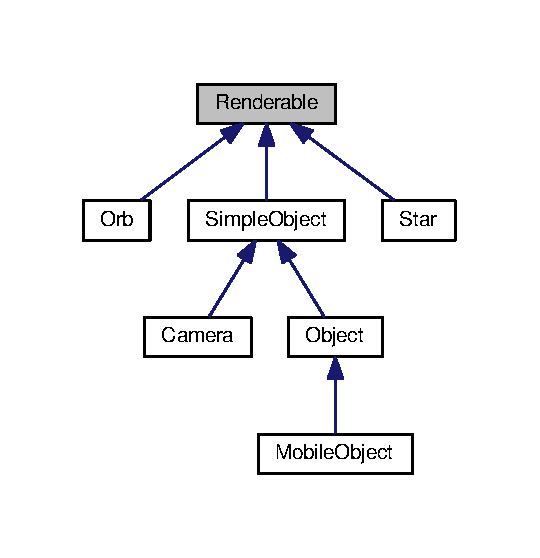
\includegraphics[width=259pt]{class_renderable__inherit__graph}
\end{center}
\end{figure}
\subsection*{Metody publiczne}
\begin{DoxyCompactItemize}
\item 
virtual bool {\bfseries is\+\_\+visible} (const \hyperlink{class_camera}{Camera} $\ast$camera)=0\hypertarget{class_renderable_a6a408454645cebdfde19ea048c488eb4}{}\label{class_renderable_a6a408454645cebdfde19ea048c488eb4}

\item 
virtual void {\bfseries render} (const \hyperlink{class_camera}{Camera} $\ast$camera)=0\hypertarget{class_renderable_ab96dd5662a667a725e7fbfeb261c9134}{}\label{class_renderable_ab96dd5662a667a725e7fbfeb261c9134}

\item 
virtual void {\bfseries update} (double dt)=0\hypertarget{class_renderable_af0588aa758ec2bf2dd476ca143167b0c}{}\label{class_renderable_af0588aa758ec2bf2dd476ca143167b0c}

\end{DoxyCompactItemize}


\subsection{Opis szczegółowy}
Klasa abstrakcyjna po której dziedziczą klasy \hyperlink{class_simple_object}{Simple\+Object}, \hyperlink{class_star}{Star} i \hyperlink{class_orb}{Orb} 

Dokumentacja dla tej klasy została wygenerowana z pliku\+:\begin{DoxyCompactItemize}
\item 
src/renderable.\+hpp\end{DoxyCompactItemize}

\hypertarget{class_simple_object}{}\section{Dokumentacja klasy Simple\+Object}
\label{class_simple_object}\index{Simple\+Object@{Simple\+Object}}


{\ttfamily \#include $<$simple\+\_\+object.\+hpp$>$}



Diagram dziedziczenia dla Simple\+Object
\nopagebreak
\begin{figure}[H]
\begin{center}
\leavevmode
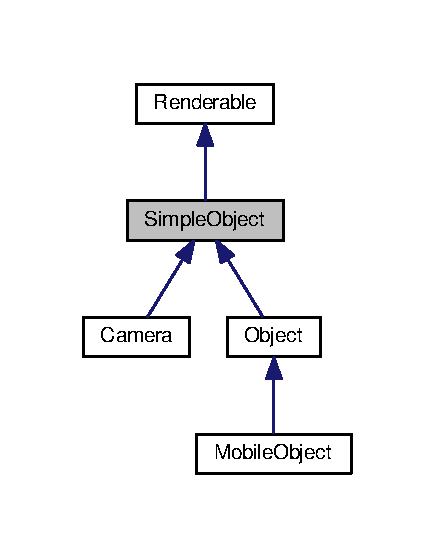
\includegraphics[width=209pt]{class_simple_object__inherit__graph}
\end{center}
\end{figure}


Diagram współpracy dla Simple\+Object\+:
\nopagebreak
\begin{figure}[H]
\begin{center}
\leavevmode
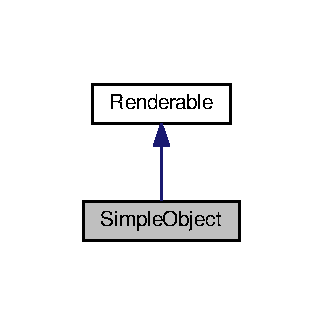
\includegraphics[width=155pt]{class_simple_object__coll__graph}
\end{center}
\end{figure}
\subsection*{Metody publiczne}
\begin{DoxyCompactItemize}
\item 
\hyperlink{class_simple_object_ac3546137e54ecbd63af642987ed7c3e1}{Simple\+Object} (double x, double y, double z, double yaw, double pitch, double roll)
\item 
\hyperlink{class_simple_object_aa5c0c6312bf39207eccbe3816218c16c}{Simple\+Object} (const \hyperlink{class_object}{Object} $\ast$object)
\item 
virtual bool {\bfseries is\+\_\+visible} (const \hyperlink{class_camera}{Camera} $\ast$camera)\hypertarget{class_simple_object_a1ecfe7d2d9f54db74b5add72bde4722f}{}\label{class_simple_object_a1ecfe7d2d9f54db74b5add72bde4722f}

\item 
virtual void {\bfseries render} (const \hyperlink{class_camera}{Camera} $\ast$camera)\hypertarget{class_simple_object_a3a27ab5c46fb29fe77bd7e8bd6a3f363}{}\label{class_simple_object_a3a27ab5c46fb29fe77bd7e8bd6a3f363}

\item 
virtual void {\bfseries update} (double dt)=0\hypertarget{class_simple_object_ae6172a3cb957cb595fd77effbb051bde}{}\label{class_simple_object_ae6172a3cb957cb595fd77effbb051bde}

\item 
virtual void \hyperlink{class_simple_object_a87202d586ed9a3c115dedcad2911f7b7}{rotate\+\_\+yaw} (double Dyaw)
\item 
virtual void \hyperlink{class_simple_object_aaf69740e2c939f7e0b51924a89422f0c}{rotate\+\_\+pitch} (double Dpitch)
\item 
virtual void \hyperlink{class_simple_object_ae2df7e8abff1303b55f559102b08a2c5}{rotate\+\_\+roll} (double Droll)
\item 
double \hyperlink{class_simple_object_a41bbdfe52dc20d88ba6511208867d908}{get\+\_\+x} () const 
\item 
double \hyperlink{class_simple_object_ac1f8fa29e45089a4110848ddaf440322}{get\+\_\+y} () const 
\item 
double \hyperlink{class_simple_object_a4a7931d70d156e0254d3ccfa1a6f2f4d}{get\+\_\+z} () const 
\item 
void \hyperlink{class_simple_object_a4c07cb27c02089325fd65dee3218563c}{move\+\_\+x} (double dx)
\item 
void \hyperlink{class_simple_object_acb544eaea6d132ddf29db57ada174920}{move\+\_\+y} (double dy)
\item 
void \hyperlink{class_simple_object_a9d5854c99305702d0b1ceaf7a24907fc}{move\+\_\+z} (double dz)
\item 
double \hyperlink{class_simple_object_a5fdb2d7aa58fcad8acb1fcaf906dce15}{get\+\_\+yaw} () const 
\item 
double \hyperlink{class_simple_object_a5fdf130ef90fe9a645887f6735f2ce70}{get\+\_\+pitch} () const 
\item 
double \hyperlink{class_simple_object_adf120ce1354dbbaed33b437206936541}{get\+\_\+roll} () const 
\end{DoxyCompactItemize}
\subsection*{Atrybuty chronione}
\begin{DoxyCompactItemize}
\item 
double {\bfseries x\+\_\+}\hypertarget{class_simple_object_a5ef9c7a8f7fb8ac661bff5dcb33983a7}{}\label{class_simple_object_a5ef9c7a8f7fb8ac661bff5dcb33983a7}

\item 
double {\bfseries y\+\_\+}\hypertarget{class_simple_object_ac80d26a13b1c0bd55403a947745b5f03}{}\label{class_simple_object_ac80d26a13b1c0bd55403a947745b5f03}

\item 
double {\bfseries z\+\_\+}\hypertarget{class_simple_object_a7adae5ef28bc1101e6a0341f1b97f4cd}{}\label{class_simple_object_a7adae5ef28bc1101e6a0341f1b97f4cd}

\item 
double {\bfseries yaw\+\_\+}\hypertarget{class_simple_object_a2223327221cd21410ac4d60fa1ad479a}{}\label{class_simple_object_a2223327221cd21410ac4d60fa1ad479a}

\item 
double {\bfseries pitch\+\_\+}\hypertarget{class_simple_object_aa4966ef233fe74cc77c0a75e97729221}{}\label{class_simple_object_aa4966ef233fe74cc77c0a75e97729221}

\item 
double {\bfseries roll\+\_\+}\hypertarget{class_simple_object_ae253b25a26259913b424129021885911}{}\label{class_simple_object_ae253b25a26259913b424129021885911}

\end{DoxyCompactItemize}
\subsection*{Przyjaciele}
\begin{DoxyCompactItemize}
\item 
double \hyperlink{class_simple_object_adbeedfd57e99d5aeab512c85ee1b6849}{calculate\+\_\+distance} (const \hyperlink{class_simple_object}{Simple\+Object} $\ast$o1, const \hyperlink{class_simple_object}{Simple\+Object} $\ast$o2)
\end{DoxyCompactItemize}


\subsection{Opis szczegółowy}
Klasa abstrakcyjna po której dziedziczą klasy \hyperlink{class_object}{Object} i \hyperlink{class_camera}{Camera} 

\subsection{Dokumentacja konstruktora i destruktora}
\index{Simple\+Object@{Simple\+Object}!Simple\+Object@{Simple\+Object}}
\index{Simple\+Object@{Simple\+Object}!Simple\+Object@{Simple\+Object}}
\subsubsection[{\texorpdfstring{Simple\+Object(double x, double y, double z, double yaw, double pitch, double roll)}{SimpleObject(double x, double y, double z, double yaw, double pitch, double roll)}}]{\setlength{\rightskip}{0pt plus 5cm}Simple\+Object\+::\+Simple\+Object (
\begin{DoxyParamCaption}
\item[{double}]{x, }
\item[{double}]{y, }
\item[{double}]{z, }
\item[{double}]{yaw = {\ttfamily 0.0}, }
\item[{double}]{pitch = {\ttfamily 0.0}, }
\item[{double}]{roll = {\ttfamily 0.0}}
\end{DoxyParamCaption}
)}\hypertarget{class_simple_object_ac3546137e54ecbd63af642987ed7c3e1}{}\label{class_simple_object_ac3546137e54ecbd63af642987ed7c3e1}
Konstruktor klasy \hyperlink{class_simple_object}{Simple\+Object} 
\begin{DoxyParams}{Parametry}
{\em x} & -\/ położenie w osi x \\
\hline
{\em y} & -\/ położenie w osi y \\
\hline
{\em z} & -\/ położenie w osi z \\
\hline
{\em yaw} & -\/ obrót w osi z \\
\hline
{\em pitch} & -\/ obrót w osi xy \\
\hline
{\em roll} & -\/ obrót wokół własnej osi \\
\hline
\end{DoxyParams}
\begin{DoxyReturn}{Zwraca}
obiekt typu \hyperlink{class_simple_object}{Simple\+Object} 
\end{DoxyReturn}
\index{Simple\+Object@{Simple\+Object}!Simple\+Object@{Simple\+Object}}
\index{Simple\+Object@{Simple\+Object}!Simple\+Object@{Simple\+Object}}
\subsubsection[{\texorpdfstring{Simple\+Object(const Object $\ast$object)}{SimpleObject(const Object *object)}}]{\setlength{\rightskip}{0pt plus 5cm}Simple\+Object\+::\+Simple\+Object (
\begin{DoxyParamCaption}
\item[{const {\bf Object} $\ast$}]{object}
\end{DoxyParamCaption}
)}\hypertarget{class_simple_object_aa5c0c6312bf39207eccbe3816218c16c}{}\label{class_simple_object_aa5c0c6312bf39207eccbe3816218c16c}
Konstruktor kopiujący klasy \hyperlink{class_simple_object}{Simple\+Object} z klasy \hyperlink{class_object}{Object} 
\begin{DoxyParams}{Parametry}
{\em object} & -\/ referencja na obiekt z którego są kopiowane fane \\
\hline
\end{DoxyParams}
\begin{DoxyReturn}{Zwraca}
obiekt typu \hyperlink{class_simple_object}{Simple\+Object} 
\end{DoxyReturn}


\subsection{Dokumentacja funkcji składowych}
\index{Simple\+Object@{Simple\+Object}!get\+\_\+pitch@{get\+\_\+pitch}}
\index{get\+\_\+pitch@{get\+\_\+pitch}!Simple\+Object@{Simple\+Object}}
\subsubsection[{\texorpdfstring{get\+\_\+pitch() const }{get_pitch() const }}]{\setlength{\rightskip}{0pt plus 5cm}double Simple\+Object\+::get\+\_\+pitch (
\begin{DoxyParamCaption}
{}
\end{DoxyParamCaption}
) const\hspace{0.3cm}{\ttfamily [inline]}}\hypertarget{class_simple_object_a5fdf130ef90fe9a645887f6735f2ce70}{}\label{class_simple_object_a5fdf130ef90fe9a645887f6735f2ce70}
Zwraca kąt obrotu w osi xy 
\begin{DoxyParams}{Parametry}
{\em wartość} & kąta w radianach $<$-\/pi/2;pi/2$>$ \\
\hline
\end{DoxyParams}
\index{Simple\+Object@{Simple\+Object}!get\+\_\+roll@{get\+\_\+roll}}
\index{get\+\_\+roll@{get\+\_\+roll}!Simple\+Object@{Simple\+Object}}
\subsubsection[{\texorpdfstring{get\+\_\+roll() const }{get_roll() const }}]{\setlength{\rightskip}{0pt plus 5cm}double Simple\+Object\+::get\+\_\+roll (
\begin{DoxyParamCaption}
{}
\end{DoxyParamCaption}
) const\hspace{0.3cm}{\ttfamily [inline]}}\hypertarget{class_simple_object_adf120ce1354dbbaed33b437206936541}{}\label{class_simple_object_adf120ce1354dbbaed33b437206936541}
Zwraca kąt obrotu wokół własnej osi 
\begin{DoxyParams}{Parametry}
{\em wartość} & kąta w radianach $<$-\/pi;pi$>$ \\
\hline
\end{DoxyParams}
\index{Simple\+Object@{Simple\+Object}!get\+\_\+x@{get\+\_\+x}}
\index{get\+\_\+x@{get\+\_\+x}!Simple\+Object@{Simple\+Object}}
\subsubsection[{\texorpdfstring{get\+\_\+x() const }{get_x() const }}]{\setlength{\rightskip}{0pt plus 5cm}double Simple\+Object\+::get\+\_\+x (
\begin{DoxyParamCaption}
{}
\end{DoxyParamCaption}
) const\hspace{0.3cm}{\ttfamily [inline]}}\hypertarget{class_simple_object_a41bbdfe52dc20d88ba6511208867d908}{}\label{class_simple_object_a41bbdfe52dc20d88ba6511208867d908}
zwraca wartość składowej x \begin{DoxyReturn}{Zwraca}
składowa x 
\end{DoxyReturn}
\index{Simple\+Object@{Simple\+Object}!get\+\_\+y@{get\+\_\+y}}
\index{get\+\_\+y@{get\+\_\+y}!Simple\+Object@{Simple\+Object}}
\subsubsection[{\texorpdfstring{get\+\_\+y() const }{get_y() const }}]{\setlength{\rightskip}{0pt plus 5cm}double Simple\+Object\+::get\+\_\+y (
\begin{DoxyParamCaption}
{}
\end{DoxyParamCaption}
) const\hspace{0.3cm}{\ttfamily [inline]}}\hypertarget{class_simple_object_ac1f8fa29e45089a4110848ddaf440322}{}\label{class_simple_object_ac1f8fa29e45089a4110848ddaf440322}
zwraca wartość składowej y \begin{DoxyReturn}{Zwraca}
składowa y 
\end{DoxyReturn}
\index{Simple\+Object@{Simple\+Object}!get\+\_\+yaw@{get\+\_\+yaw}}
\index{get\+\_\+yaw@{get\+\_\+yaw}!Simple\+Object@{Simple\+Object}}
\subsubsection[{\texorpdfstring{get\+\_\+yaw() const }{get_yaw() const }}]{\setlength{\rightskip}{0pt plus 5cm}double Simple\+Object\+::get\+\_\+yaw (
\begin{DoxyParamCaption}
{}
\end{DoxyParamCaption}
) const\hspace{0.3cm}{\ttfamily [inline]}}\hypertarget{class_simple_object_a5fdb2d7aa58fcad8acb1fcaf906dce15}{}\label{class_simple_object_a5fdb2d7aa58fcad8acb1fcaf906dce15}
Zwraca kąt obrotu w osi z 
\begin{DoxyParams}{Parametry}
{\em wartość} & kąta w radianach $<$-\/pi;pi$>$ \\
\hline
\end{DoxyParams}
\index{Simple\+Object@{Simple\+Object}!get\+\_\+z@{get\+\_\+z}}
\index{get\+\_\+z@{get\+\_\+z}!Simple\+Object@{Simple\+Object}}
\subsubsection[{\texorpdfstring{get\+\_\+z() const }{get_z() const }}]{\setlength{\rightskip}{0pt plus 5cm}double Simple\+Object\+::get\+\_\+z (
\begin{DoxyParamCaption}
{}
\end{DoxyParamCaption}
) const\hspace{0.3cm}{\ttfamily [inline]}}\hypertarget{class_simple_object_a4a7931d70d156e0254d3ccfa1a6f2f4d}{}\label{class_simple_object_a4a7931d70d156e0254d3ccfa1a6f2f4d}
zwraca wartość składowej z \begin{DoxyReturn}{Zwraca}
składowa z 
\end{DoxyReturn}
\index{Simple\+Object@{Simple\+Object}!move\+\_\+x@{move\+\_\+x}}
\index{move\+\_\+x@{move\+\_\+x}!Simple\+Object@{Simple\+Object}}
\subsubsection[{\texorpdfstring{move\+\_\+x(double dx)}{move_x(double dx)}}]{\setlength{\rightskip}{0pt plus 5cm}void Simple\+Object\+::move\+\_\+x (
\begin{DoxyParamCaption}
\item[{double}]{dx}
\end{DoxyParamCaption}
)\hspace{0.3cm}{\ttfamily [inline]}}\hypertarget{class_simple_object_a4c07cb27c02089325fd65dee3218563c}{}\label{class_simple_object_a4c07cb27c02089325fd65dee3218563c}
Przesuwa w osi x 
\begin{DoxyParams}{Parametry}
{\em dx} & -\/ wartość przesunięcia \\
\hline
\end{DoxyParams}
\index{Simple\+Object@{Simple\+Object}!move\+\_\+y@{move\+\_\+y}}
\index{move\+\_\+y@{move\+\_\+y}!Simple\+Object@{Simple\+Object}}
\subsubsection[{\texorpdfstring{move\+\_\+y(double dy)}{move_y(double dy)}}]{\setlength{\rightskip}{0pt plus 5cm}void Simple\+Object\+::move\+\_\+y (
\begin{DoxyParamCaption}
\item[{double}]{dy}
\end{DoxyParamCaption}
)\hspace{0.3cm}{\ttfamily [inline]}}\hypertarget{class_simple_object_acb544eaea6d132ddf29db57ada174920}{}\label{class_simple_object_acb544eaea6d132ddf29db57ada174920}
Przesuwa w osi y 
\begin{DoxyParams}{Parametry}
{\em dy} & -\/ wartość przesunięcia \\
\hline
\end{DoxyParams}
\index{Simple\+Object@{Simple\+Object}!move\+\_\+z@{move\+\_\+z}}
\index{move\+\_\+z@{move\+\_\+z}!Simple\+Object@{Simple\+Object}}
\subsubsection[{\texorpdfstring{move\+\_\+z(double dz)}{move_z(double dz)}}]{\setlength{\rightskip}{0pt plus 5cm}void Simple\+Object\+::move\+\_\+z (
\begin{DoxyParamCaption}
\item[{double}]{dz}
\end{DoxyParamCaption}
)\hspace{0.3cm}{\ttfamily [inline]}}\hypertarget{class_simple_object_a9d5854c99305702d0b1ceaf7a24907fc}{}\label{class_simple_object_a9d5854c99305702d0b1ceaf7a24907fc}
Przesuwa w osi z 
\begin{DoxyParams}{Parametry}
{\em dx=z} & -\/ wartość przesunięcia \\
\hline
\end{DoxyParams}
\index{Simple\+Object@{Simple\+Object}!rotate\+\_\+pitch@{rotate\+\_\+pitch}}
\index{rotate\+\_\+pitch@{rotate\+\_\+pitch}!Simple\+Object@{Simple\+Object}}
\subsubsection[{\texorpdfstring{rotate\+\_\+pitch(double Dpitch)}{rotate_pitch(double Dpitch)}}]{\setlength{\rightskip}{0pt plus 5cm}void Simple\+Object\+::rotate\+\_\+pitch (
\begin{DoxyParamCaption}
\item[{double}]{Dpitch}
\end{DoxyParamCaption}
)\hspace{0.3cm}{\ttfamily [virtual]}}\hypertarget{class_simple_object_aaf69740e2c939f7e0b51924a89422f0c}{}\label{class_simple_object_aaf69740e2c939f7e0b51924a89422f0c}
Obraca w osi xy o zadany kąt i przelicza go na wartość z zakresu $<$-\/pi/2;pi/2$>$ uwzględniając wpływ na obrót w pozostałych dwóch osiach 
\begin{DoxyParams}{Parametry}
{\em Dpitch} & -\/ wartość przesunięcia \\
\hline
\end{DoxyParams}
\index{Simple\+Object@{Simple\+Object}!rotate\+\_\+roll@{rotate\+\_\+roll}}
\index{rotate\+\_\+roll@{rotate\+\_\+roll}!Simple\+Object@{Simple\+Object}}
\subsubsection[{\texorpdfstring{rotate\+\_\+roll(double Droll)}{rotate_roll(double Droll)}}]{\setlength{\rightskip}{0pt plus 5cm}void Simple\+Object\+::rotate\+\_\+roll (
\begin{DoxyParamCaption}
\item[{double}]{Droll}
\end{DoxyParamCaption}
)\hspace{0.3cm}{\ttfamily [virtual]}}\hypertarget{class_simple_object_ae2df7e8abff1303b55f559102b08a2c5}{}\label{class_simple_object_ae2df7e8abff1303b55f559102b08a2c5}
Obraca w osi obiektu o zadany kąt i przelicza go na wartość z zakresu $<$-\/pi;pi$>$ 
\begin{DoxyParams}{Parametry}
{\em Droll} & -\/ wartość przesunięcia \\
\hline
\end{DoxyParams}
\index{Simple\+Object@{Simple\+Object}!rotate\+\_\+yaw@{rotate\+\_\+yaw}}
\index{rotate\+\_\+yaw@{rotate\+\_\+yaw}!Simple\+Object@{Simple\+Object}}
\subsubsection[{\texorpdfstring{rotate\+\_\+yaw(double Dyaw)}{rotate_yaw(double Dyaw)}}]{\setlength{\rightskip}{0pt plus 5cm}void Simple\+Object\+::rotate\+\_\+yaw (
\begin{DoxyParamCaption}
\item[{double}]{Dyaw}
\end{DoxyParamCaption}
)\hspace{0.3cm}{\ttfamily [virtual]}}\hypertarget{class_simple_object_a87202d586ed9a3c115dedcad2911f7b7}{}\label{class_simple_object_a87202d586ed9a3c115dedcad2911f7b7}
Obraca w osi z o zadany kąt i przelicza go na wartość z zakresu $<$-\/pi;pi$>$ 
\begin{DoxyParams}{Parametry}
{\em Dyaw} & -\/ wartość przesunięcia \\
\hline
\end{DoxyParams}


\subsection{Dokumentacja przyjaciół i funkcji związanych}
\index{Simple\+Object@{Simple\+Object}!calculate\+\_\+distance@{calculate\+\_\+distance}}
\index{calculate\+\_\+distance@{calculate\+\_\+distance}!Simple\+Object@{Simple\+Object}}
\subsubsection[{\texorpdfstring{calculate\+\_\+distance}{calculate_distance}}]{\setlength{\rightskip}{0pt plus 5cm}double calculate\+\_\+distance (
\begin{DoxyParamCaption}
\item[{const {\bf Simple\+Object} $\ast$}]{o1, }
\item[{const {\bf Simple\+Object} $\ast$}]{o2}
\end{DoxyParamCaption}
)\hspace{0.3cm}{\ttfamily [friend]}}\hypertarget{class_simple_object_adbeedfd57e99d5aeab512c85ee1b6849}{}\label{class_simple_object_adbeedfd57e99d5aeab512c85ee1b6849}
Oblicza odległość między dwoma obiektami 
\begin{DoxyParams}{Parametry}
{\em o1} & -\/ wskaźnik na pierwszy obiekt \\
\hline
{\em o2} & -\/ wskaźnik na drugi obiekt \\
\hline
\end{DoxyParams}
\begin{DoxyReturn}{Zwraca}
odległość w kilometrach 
\end{DoxyReturn}


Dokumentacja dla tej klasy została wygenerowana z plików\+:\begin{DoxyCompactItemize}
\item 
src/simple\+\_\+object.\+hpp\item 
src/simple\+\_\+object.\+cpp\end{DoxyCompactItemize}

\hypertarget{class_simulator}{}\section{Simulator Class Reference}
\label{class_simulator}\index{Simulator@{Simulator}}


{\ttfamily \#include $<$multi.\+hpp$>$}

\subsection*{Public Member Functions}
\begin{DoxyCompactItemize}
\item 
\hyperlink{class_simulator_a597385e2e9f501fbbd936e3b281cd2b1}{Simulator} (std\+::vector$<$ \hyperlink{class_renderable}{Renderable} $\ast$ $>$ simulatables, double dt)
\item 
void \hyperlink{class_simulator_ab844c2061cc955301bd63016e67ed2e0}{operator()} ()
\item 
void \hyperlink{class_simulator_a21d308aa878b8a23482a00d8939a9ada}{update\+\_\+buffer} ()
\item 
std\+::vector$<$ \hyperlink{class_renderable}{Renderable} $\ast$ $>$ \hyperlink{class_simulator_a276673b4c7124e93d037f8b0e857ea11}{get\+\_\+buffer} ()
\end{DoxyCompactItemize}


\subsection{Detailed Description}
Klasa odpowiedzialna za prowadzenie symulacji w osobnym wątku (T\+BA). 

\subsection{Constructor \& Destructor Documentation}
\index{Simulator@{Simulator}!Simulator@{Simulator}}
\index{Simulator@{Simulator}!Simulator@{Simulator}}
\subsubsection[{\texorpdfstring{Simulator(std\+::vector$<$ Renderable $\ast$ $>$ simulatables, double dt)}{Simulator(std::vector< Renderable * > simulatables, double dt)}}]{\setlength{\rightskip}{0pt plus 5cm}Simulator\+::\+Simulator (
\begin{DoxyParamCaption}
\item[{std\+::vector$<$ {\bf Renderable} $\ast$ $>$}]{simulatables, }
\item[{double}]{dt}
\end{DoxyParamCaption}
)}\hypertarget{class_simulator_a597385e2e9f501fbbd936e3b281cd2b1}{}\label{class_simulator_a597385e2e9f501fbbd936e3b281cd2b1}
Konstruktor klasy \hyperlink{class_simulator}{Simulator} 
\begin{DoxyParams}{Parameters}
{\em simulatables} & -\/ tablica wskaźników na obiekty które mają być symulowane \\
\hline
{\em dt} & -\/ krok czasowy symulacji \\
\hline
\end{DoxyParams}
\begin{DoxyReturn}{Returns}
obiekt klasy \hyperlink{class_simulator}{Simulator} 
\end{DoxyReturn}


\subsection{Member Function Documentation}
\index{Simulator@{Simulator}!get\+\_\+buffer@{get\+\_\+buffer}}
\index{get\+\_\+buffer@{get\+\_\+buffer}!Simulator@{Simulator}}
\subsubsection[{\texorpdfstring{get\+\_\+buffer()}{get_buffer()}}]{\setlength{\rightskip}{0pt plus 5cm}std\+::vector$<${\bf Renderable}$\ast$$>$ Simulator\+::get\+\_\+buffer (
\begin{DoxyParamCaption}
{}
\end{DoxyParamCaption}
)\hspace{0.3cm}{\ttfamily [inline]}}\hypertarget{class_simulator_a276673b4c7124e93d037f8b0e857ea11}{}\label{class_simulator_a276673b4c7124e93d037f8b0e857ea11}
Zwraca bufor dla wątku renderującego \begin{DoxyReturn}{Returns}
kopia bufora 
\end{DoxyReturn}
\index{Simulator@{Simulator}!operator()@{operator()}}
\index{operator()@{operator()}!Simulator@{Simulator}}
\subsubsection[{\texorpdfstring{operator()()}{operator()()}}]{\setlength{\rightskip}{0pt plus 5cm}void Simulator\+::operator() (
\begin{DoxyParamCaption}
{}
\end{DoxyParamCaption}
)}\hypertarget{class_simulator_ab844c2061cc955301bd63016e67ed2e0}{}\label{class_simulator_ab844c2061cc955301bd63016e67ed2e0}
Wątek w którym trwa symulacja \index{Simulator@{Simulator}!update\+\_\+buffer@{update\+\_\+buffer}}
\index{update\+\_\+buffer@{update\+\_\+buffer}!Simulator@{Simulator}}
\subsubsection[{\texorpdfstring{update\+\_\+buffer()}{update_buffer()}}]{\setlength{\rightskip}{0pt plus 5cm}void Simulator\+::update\+\_\+buffer (
\begin{DoxyParamCaption}
{}
\end{DoxyParamCaption}
)\hspace{0.3cm}{\ttfamily [inline]}}\hypertarget{class_simulator_a21d308aa878b8a23482a00d8939a9ada}{}\label{class_simulator_a21d308aa878b8a23482a00d8939a9ada}
Aktualizuje bufor do zwracania do wątku renderującego 

The documentation for this class was generated from the following files\+:\begin{DoxyCompactItemize}
\item 
src/multi.\+hpp\item 
src/multi.\+cpp\end{DoxyCompactItemize}

\hypertarget{class_star}{}\section{Star Class Reference}
\label{class_star}\index{Star@{Star}}


{\ttfamily \#include $<$star.\+hpp$>$}



Inheritance diagram for Star\+:\nopagebreak
\begin{figure}[H]
\begin{center}
\leavevmode
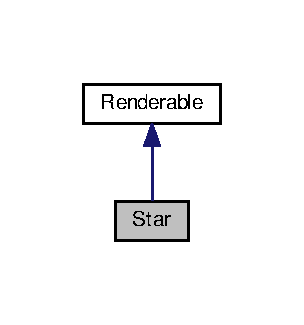
\includegraphics[width=146pt]{class_star__inherit__graph}
\end{center}
\end{figure}


Collaboration diagram for Star\+:\nopagebreak
\begin{figure}[H]
\begin{center}
\leavevmode
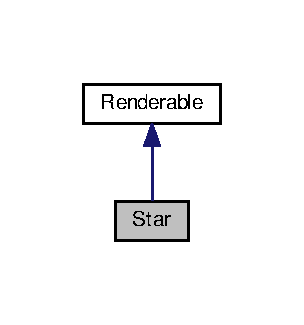
\includegraphics[width=146pt]{class_star__coll__graph}
\end{center}
\end{figure}
\subsection*{Public Member Functions}
\begin{DoxyCompactItemize}
\item 
\hyperlink{class_star_ac79a6fb3556d6735f063cbc28fb73397}{Star} (double alfa=0, double beta=0)
\item 
\hyperlink{class_star_a125afff584b315791b7345151f978c99}{Star} (double alfa, double beta, uint\+\_\+fast8\+\_\+t r, uint\+\_\+fast8\+\_\+t g\+\_\+, uint\+\_\+fast8\+\_\+t b\+\_\+)
\item 
virtual void {\bfseries update} (double dt)\hypertarget{class_star_a6329b84f6a4434f93f744475336758da}{}\label{class_star_a6329b84f6a4434f93f744475336758da}

\item 
virtual bool \hyperlink{class_star_ac196fa232107776abeddba91ccdc3374}{is\+\_\+visible} (const \hyperlink{class_camera}{Camera} $\ast$camera)
\item 
virtual void \hyperlink{class_star_af0cb257b2c6e44cd26d75113e5e6675d}{render} (const \hyperlink{class_camera}{Camera} $\ast$camera)
\end{DoxyCompactItemize}
\subsection*{Protected Attributes}
\begin{DoxyCompactItemize}
\item 
double {\bfseries alfa\+\_\+}\hypertarget{class_star_acbc2ce5b635761779c628b82eebaa914}{}\label{class_star_acbc2ce5b635761779c628b82eebaa914}

\item 
double {\bfseries beta\+\_\+}\hypertarget{class_star_ac560d7b5ff53fea9b4c816bd0104fe9a}{}\label{class_star_ac560d7b5ff53fea9b4c816bd0104fe9a}

\item 
uint\+\_\+fast8\+\_\+t {\bfseries r\+\_\+}\hypertarget{class_star_afc7dd12c9f1876daec0d8900310df9d3}{}\label{class_star_afc7dd12c9f1876daec0d8900310df9d3}

\item 
uint\+\_\+fast8\+\_\+t {\bfseries g\+\_\+}\hypertarget{class_star_afacfcae0967a657fe5764e78439c2e57}{}\label{class_star_afacfcae0967a657fe5764e78439c2e57}

\item 
uint\+\_\+fast8\+\_\+t {\bfseries b\+\_\+}\hypertarget{class_star_abd9108ee6d13e26ef4a220777c2f40fa}{}\label{class_star_abd9108ee6d13e26ef4a220777c2f40fa}

\end{DoxyCompactItemize}


\subsection{Detailed Description}
Klasa odpowiedzialna za gwiazdy w tle 

\subsection{Constructor \& Destructor Documentation}
\index{Star@{Star}!Star@{Star}}
\index{Star@{Star}!Star@{Star}}
\subsubsection[{\texorpdfstring{Star(double alfa=0, double beta=0)}{Star(double alfa=0, double beta=0)}}]{\setlength{\rightskip}{0pt plus 5cm}Star\+::\+Star (
\begin{DoxyParamCaption}
\item[{double}]{alfa = {\ttfamily 0}, }
\item[{double}]{beta = {\ttfamily 0}}
\end{DoxyParamCaption}
)}\hypertarget{class_star_ac79a6fb3556d6735f063cbc28fb73397}{}\label{class_star_ac79a6fb3556d6735f063cbc28fb73397}
Konstruktor domyślny klasy \hyperlink{class_star}{Star} przyjmuje kolor biały 
\begin{DoxyParams}{Parameters}
{\em alfa} & -\/ kąt alfa współrzędnych sferycznych \\
\hline
{\em beta} & -\/ kąt beta współrzędnych sferycznych \\
\hline
\end{DoxyParams}
\begin{DoxyReturn}{Returns}
-\/ obiekt typu \hyperlink{class_star}{Star} koloru białego 
\end{DoxyReturn}
\index{Star@{Star}!Star@{Star}}
\index{Star@{Star}!Star@{Star}}
\subsubsection[{\texorpdfstring{Star(double alfa, double beta, uint\+\_\+fast8\+\_\+t r, uint\+\_\+fast8\+\_\+t g\+\_\+, uint\+\_\+fast8\+\_\+t b\+\_\+)}{Star(double alfa, double beta, uint_fast8_t r, uint_fast8_t g_, uint_fast8_t b_)}}]{\setlength{\rightskip}{0pt plus 5cm}Star\+::\+Star (
\begin{DoxyParamCaption}
\item[{double}]{alfa, }
\item[{double}]{beta, }
\item[{uint\+\_\+fast8\+\_\+t}]{r, }
\item[{uint\+\_\+fast8\+\_\+t}]{g, }
\item[{uint\+\_\+fast8\+\_\+t}]{b}
\end{DoxyParamCaption}
)}\hypertarget{class_star_a125afff584b315791b7345151f978c99}{}\label{class_star_a125afff584b315791b7345151f978c99}
Konstruktor domyślny klasy \hyperlink{class_star}{Star} pozwalający podać składowe kolorów 
\begin{DoxyParams}{Parameters}
{\em alfa} & -\/ kąt alfa współrzędnych sferycznych \\
\hline
{\em beta} & -\/ kąt beta współrzędnych sferycznych \\
\hline
{\em r} & -\/ składowa czerwona koloru \\
\hline
{\em g} & -\/ składowa zielona koloru \\
\hline
{\em b} & -\/ składowa niebieska koloru \\
\hline
\end{DoxyParams}
\begin{DoxyReturn}{Returns}
-\/ obiekt typu \hyperlink{class_star}{Star} 
\end{DoxyReturn}


\subsection{Member Function Documentation}
\index{Star@{Star}!is\+\_\+visible@{is\+\_\+visible}}
\index{is\+\_\+visible@{is\+\_\+visible}!Star@{Star}}
\subsubsection[{\texorpdfstring{is\+\_\+visible(const Camera $\ast$camera)}{is_visible(const Camera *camera)}}]{\setlength{\rightskip}{0pt plus 5cm}bool Star\+::is\+\_\+visible (
\begin{DoxyParamCaption}
\item[{const {\bf Camera} $\ast$}]{camera}
\end{DoxyParamCaption}
)\hspace{0.3cm}{\ttfamily [virtual]}}\hypertarget{class_star_ac196fa232107776abeddba91ccdc3374}{}\label{class_star_ac196fa232107776abeddba91ccdc3374}
Sprawdza czy gwiazda jest w polu widzenia kamery 
\begin{DoxyParams}{Parameters}
{\em camera} & -\/ wskaźnik na kamerę \\
\hline
\end{DoxyParams}
\begin{DoxyReturn}{Returns}
fałsz -\/ jeśli gwiazda jest poza polem widzenia 
\end{DoxyReturn}


Implements \hyperlink{class_renderable}{Renderable}.

\index{Star@{Star}!render@{render}}
\index{render@{render}!Star@{Star}}
\subsubsection[{\texorpdfstring{render(const Camera $\ast$camera)}{render(const Camera *camera)}}]{\setlength{\rightskip}{0pt plus 5cm}void Star\+::render (
\begin{DoxyParamCaption}
\item[{const {\bf Camera} $\ast$}]{camera}
\end{DoxyParamCaption}
)\hspace{0.3cm}{\ttfamily [virtual]}}\hypertarget{class_star_af0cb257b2c6e44cd26d75113e5e6675d}{}\label{class_star_af0cb257b2c6e44cd26d75113e5e6675d}
Rysuje gwiazdę w polu widzenia kamery 
\begin{DoxyParams}{Parameters}
{\em camera} & -\/ wskaźnik na kamerę \\
\hline
\end{DoxyParams}


Implements \hyperlink{class_renderable}{Renderable}.



The documentation for this class was generated from the following files\+:\begin{DoxyCompactItemize}
\item 
src/star.\+hpp\item 
src/star.\+cpp\end{DoxyCompactItemize}

%--- End generated contents ---

% Index
\backmatter
\newpage
\phantomsection
\clearemptydoublepage
\addcontentsline{toc}{chapter}{Index}
\printindex

\end{document}
